\documentclass[a4paper,11pt]{article}
\usepackage{a4wide}
\usepackage[ansinew]{inputenc}
\usepackage{graphicx}
\usepackage{bm}
\usepackage{natbib}
\usepackage{longtable}
\usepackage{rotating}
\usepackage{pdflscape}
%\usepackage{pdfdraftcopy}


%\usepackage{jurabib}
   %\jurabibsetup{  
     %authorformat=and  
    % commabeforerest,  
    % titleformat=colonsep,  
    % bibformat=tabular  
   %}  

\usepackage[bookmarks=true, bookmarksopen=true,
                bookmarksnumbered=true, colorlinks,citecolor = blue,
                filecolor=blue, linkcolor=blue, urlcolor=blue,
                plainpages=false,hyperindex=true]{hyperref}
\hypersetup{
        pdftitle={},
        pdfauthor={Anton Burger and Robert Ferstl},
        pdfsubject={},
        pdfkeywords={},
        pdfcreator={},
        pdfproducer={}
     }

%\usepackage{natbib}
%\usepackage{dingbat}
\usepackage{amssymb,amsmath,amstext}
%\usepackage{manfnt}

\setlength{\parindent}{0.0cm}                      % Absatzeinr�ckungen
\setlength{\parskip}{1.5ex plus 0.5ex minus 0.5ex} % Absatzabst�nde
%\renewcommand{\arraystretch}{1.5}                 % Zeilenabstand in Tabellen


\begin{document}
\title{Generation Capacity Investment in Electricity Markets \\ in an Oligopolistic, Dynamic and Stochastic Framework\\\vspace{0.3cm}\emph{Draft version}}
\author{Anton Burger\thanks{\href{http://www.wu-wien.ac.at/regulierung}{Institute for Regulatory Economics, Vienna University of Economics and Business Administration,} \href{mailto:anton.burger@wu-wien.ac.at}{anton.burger@wu-wien.ac.at}}\hspace{1cm} Robert Ferstl\thanks{\href{http://www-finanzierung.uni-regensburg.de/}{Department of Finance, University of Regensburg,} \href{mailto:robert.ferstl@wiwi.uni-regensburg.de}{robert.ferstl@wiwi.uni-regensburg.de}}}
\maketitle
\abstract{
The paper discusses game theoretic models for generation capacity investment decisions in a deregulated electricity market. The possible problem formulations involve open-loop, closed-loop and $S$-adapted Cournot equilibria. We present an example of an S-adapted Cournot equilibrium, which we apply to the German electricity market. Investment decisions derived by this dynamic oligopoly model are then compared to what the perfect competition result in an otherwise unchanged setup would be. We conclude that there seems to be a problem with underinvestment and technology mix in the current market structure.
\\
\\


\textbf{Keywords:} Electricity markets, Investment decisions, Stochastic oligopoly model, Sample path optimization, Stochastic programming
\\
\\
\textbf{JEL Codes:} D43, L51
}

\section{Introduction}

With the ongoing deregulation of electricity markets firms behave different in this new market setting. When investing in new generation capacity firms are faced with uncertainties related to the future demand of electricity and to the investment and production decisions of their competitors. \cite{Ventosa2005} gives an overview about decision support models used in electricity market modeling. There exist two types of equilibrium models. First, Cournout competition where the players compete in quantity and second, supply function equilibria (SFE) where the firms compete over their offer curves. What both approaches have in common is that they are based on the concept of \cite{Nash1951} equilibra, i.e. when each players strategy is the best response to its opponents actions the market has found an equilibrium. In the following, we will focus on the Cournot approach which is easier applicable to real world problems, because SFE can only be found under strong assumptions and convergence problems arise quite often.

An important aspect of a dynamic oligopoly model is the assumption about the information structure. The literature disinguishes between the following three cases \citep[see, e.g.,][]{Cellini2004}. \emph{Open-loop} equilibria only take into account the inital state variables and the time, but they do not include any strategic interaction based on the evolution of the state variables over time. They are not subgame perfect, meaning that not in all stages the strategies have to be Nash equilibria, and players must commit to their decision forever. The initial and current levels of all state variables are taken into account in a \emph{closed-loop} equilibrium. They can only be found for special cases. \cite{Murphy2005} consider a two-stage game where they interpret the close-loop game as electricity industry with a spot market, where players make an investment decision in the first stage and know how they will play against each other when producing the electricity. In a \emph{feedback} equilibrium information about the accumulated stock of each state variable at the current date is included.

There is a wide diversity of papers that deals with Cournot equilibria in the spot market for electricity \citep[see, e.g.][]{Borenstein1999, Otero-Novas2000}. Here, the strategic decision making is performed under a short time horizon. The following recent papers specifically model the investment problem in electricty markets, which clearly has a medium to long-term focus.

\cite{Chuang2001}

\cite{Ventosa2002}

\cite{Hogendorn2003}

\cite{Chaton2003}

\cite{Pineau2003} argue that electricity generators stick to their investment decisions for some time while only adjusting for shocks in exogenous variables. Therefore, they think it is possible to gain some insight in the strategic behaviour with a model based on $S$-adapted open-loop equilibria.

Electricity demand is uncertain and varies over time. The usual way to represent this fact is with a load duration curve. \cite{Murphy2005} convert the inverse to a probability density function and interpret it as a way to cope with the overall uncertainty about the future demand for electricity.

\cite{Neuhoff2005} analyze electricty markets with transmission constraints but their models are not multi-stage.

\cite{Sauma2006} evaluate social welfare implications of investments in transmission capacity. Market deregulation has lead to independent companies that operate the transmission network but may not necessarily generate the electricity. For the generators action they use a simplified version of the \cite{Murphy2005} generation capacity investment model.

\cite{Barmack2007}

\cite{Centeno2007} model medium-term strategic generation decisions based on a conjectured price-response market equilibrium.

\cite{Genc2007}

\cite{Kiesling2007}

 






\subsection{Test}
\label{sec:test}

Instead of using the optimization criterion as in stochastic programming the Nash equilibrium computation is performed over the whole sample space so that players maximize their expected profit.

In this paper we will build a model for generation capacity investment under uncertainty. We consider a deregulated electricity market, where typically several large players act on market leading to an oligopoly situation. There is not much literature which directly deals with the question of  generation capacity investments. Recent works are \cite{Chuang2001}, \cite{Ventosa2002}, \cite{Chaton2003}, \cite{Hogendorn2003}, \cite{Pineau2003}, \cite{Ehrenmann2004}. \cite{Murphy2005}, \cite{Kiesling2007}, \cite{Pineau2007}.


Cournot is more flexible and better computational tractability.


\subsection{Stochastic oligopoly models}

\textbf{References:} \cite{Salant1982, Wolf1997, Haurie2002, Pineau2003, Murto2004}\\


The $S$-adapted information structure was introduced by \cite{Haurie1990}.
$S$-adapted structure is similar to the open-loop case, except that the strategies of the players adapt to the sample path of the stochastic variable \citep[see][pg. 128]{Pineau2003}.

\cite{Haurie2002} developed an approximation method with variational inequalities for $S$-adapted oligopoly equilibria. It can be used with any discrete state process that can be represented as an event tree can be used as description of the random disturbances.

\cite{Murto2004} solves the game with feedback information structure.

\cite{Haurie2001}, \cite{Genc2007}

\subsection{Short-term assumption for decision variables}

Cournot, Bertrand, SFE


In theory, the output of a competitive generation market is equal to the output of a regulated system with a central planner that minimizes investment plus operating costs to meet demand (Green, 2000), see \citep[see][pg. 111]{Rothwell2003}.

Papers with focus investment problem: \cite{Pineau2003}, \cite{Murphy2005}, \cite{Genc2007}, \cite{Kiesling2007}, \cite{Barmack2007}, \cite{Sauma2006}

Market simulation: \cite{Torre2003}, \cite{Valenzuela2007}, \cite{Hobbs2001},\cite{Otero-Novas2000}

General review paper: \cite{Neuhoff2005}, \cite{Ventosa2005}, \cite{Kahn1998}

%%% Local Variables: 
%%% mode: latex
%%% TeX-master: "../emarket_simulation"
%%% End: 

%\section{Strategic Capacity Investments under imperfect Competition}

\subsection{The short run or open loop Game}

					\begin{frame}
					
\frametitle{The short run or open loop Game}

The duopoly Cournot model for an electricity Market from Murphy and Smeers (2005)
\begin{gather}
	\min_{x_i,y_i^s} \sum_s \left[ - \alpha^s + \beta (y_i^s+y_{-i}^s) \right] y_i^s + v_i \sum_s y_i^s + K_i x_i \\
\text{s.t.:} \  x_i-y_i^s \geq 0; \  y_i^s \geq 0; \ \nonumber
\end{gather}
{\small
\begin{tabbing}
whereby: \= $y_i^s$ \  \= output per player and demand segment \\
\> $x_i$   \    \> capacity  \\
\> $\alpha - \beta y$    \   \= inverse demand curve \\
\> $v_i, K_i$    \    \> variable and capacity costs
\end{tabbing}}
The first order conditions are:
\begin{equation}
	\frac{\partial (- \pi)}{\partial y_i^s} = -\alpha^s + 2 \beta y_i^s +  y_{-i}^s + v_i + \lambda_i^s = \omega_i^s 
\end{equation}
By using the first order condition to obtain reaction functions, the mutual best responses can be found
					\end{frame}


\subsection{Closed loop Equilibrium}

					\begin{frame}
					
\frametitle{Closed loop Equilibrium}

We have to solve the problem now, under the assumption that the quantities in the second period are a function of investments in the first period $y_i^s(x_i;x_{-i})$.

\begin{equation}
	\min_{x_i} \sum_{s=1}^S \left[ - \alpha^s + \beta( y_i^s(x_i;x_{-i})+ y_{-i}^s(x_i;x_{-i})) + v_i \right] y_i^s(x_i;x_{-i}) + K_i x_i
\end{equation}

and the solution has to satisfy the following condition:

\begin{equation}
	\frac{\partial (- \pi)}{\partial x_i} = \sum_s \left[-\alpha^s + 2 \beta y_i^s (\cdot) + \beta y_{-i}^s(\cdot) + v_i \right] \frac{\partial y_i^s (\cdot)}{\partial x_i} + \sum_s \beta y_i^s (\cdot) \frac{\partial y_{-i}^s (\cdot)}{\partial x_i} + K_i
\end{equation}

The effect of an investment of player $i$ on the action of player $-i$ in the second period $\partial y_{-i} (\cdot)/\partial x_i$ is now taken into account.


							\end{frame}
\section{Data}

The German electricity market was liberalized in 1998 and is the largest in Europe with a gross production of 633.2 TWh in 2006 \citep{IEA2007}. More than half of the power is generated with coal, other major sources are nuclear and gas. The German power market is dominated by a few large players (E.ON, RWE, EnBW, Vattenfall). These firms are both transmission system operators and own 90\% of total generation capacity. \cite{Brunekreeft2006} report values for the Herfindahl Hirschman Index (HHI)\footnote{This is a common measure of market power and is calculated as sum of the squared market shares in an industry.} of over 2000. Electricity distribution is organized by approximately 900 communal distributors. The German energy market regulator  \emph{Bundesnetzagentur} was installed in 2005. Germany decided on a phase-out of nuclear power generation by 2020. The \emph{German Energy Agency} estimates that investments in generation capacity of up to 40,000 MW will be necessary, see Fig. \ref{fig:nuclear}. Furthermore, a large stake of the existing generation capacities are close to the end of its service life. This, together with a tendency towards more environmental-friendly technologies supports the importance of strategic investments by the major players in the market. 

\begin{figure}[htb]
  \centering
\caption{Estimated nuclear power capacity, 2007 to 2023}
 % \includegraphics[width=.7\textwidth]{germandata/nuclear.pdf}
\includegraphics[width=3.5in]{germandata/nuclear.pdf}
  \label{fig:nuclear}
\\
 \scriptsize Source: \cite{IEA2007a}
\end{figure}

Tab. \ref{tab:majorcapacities} gives an overview about the existing installed capacity in different technologies.

\begin{table}[htb]
\centering
\scriptsize
\caption{Installed capacities in MW of major players in Germany}
\vspace{0.3cm}
\begin{tabular}[htb]{crrrrrrrrr}
\hline
           &      Hydro &    Nuclear &  Soft coal &  Hard coal &        Gas &        Oil &     Pumped \\
\hline\hline
       RWE &        741 &       5,499 &      10,554 &       7,249 &       4,297 &        188 &        793 \\

      E.ON &       1,320 &       8,473 &       1,425 &       9,461 &       3,808 &       1,779 &       1,110 \\

Vattenfall &          9 &       1,421 &       6,932 &       1,729 &        870 &       1,429 &       2,883 \\

      EnBW &        447 &       4,272 &        453 &       3,288 &       1,083 &        617 &        368 \\
\hline
\end{tabular} 
\label{tab:majorcapacities}
\\
\vspace{0.3cm}
\scriptsize Source: \cite{Ellersdorfer2005}
\end{table}

%Figure \ref{fig:investcosts} contains investment costs for different technologies.

%\begin{figure}[htb]
%  \centering
%\caption{Levelised costs for generation units starting commercial operation in 2015}
%  \includegraphics[width=.5\textwidth]{germandata/investmentcosts.pdf}
%  \label{fig:investcosts}
%\\
% \scriptsize Source: \cite{IEA2007c}
%\end{figure}

The major stake of electricity trading is done in OTC markets for which it is hard to obtain data. Prices from the European Energy Exchange (EEX) can be used as a good approximation. Plotting the prices against the trading volumes does not show a strong correlation. We see the expected positive relationship when comparing the exchange prices to the actual electricity demand per hour, see Fig. \ref{fig:pricequant}

\begin{figure}[htb]
  \centering
\caption{Price-quantity relationship}
  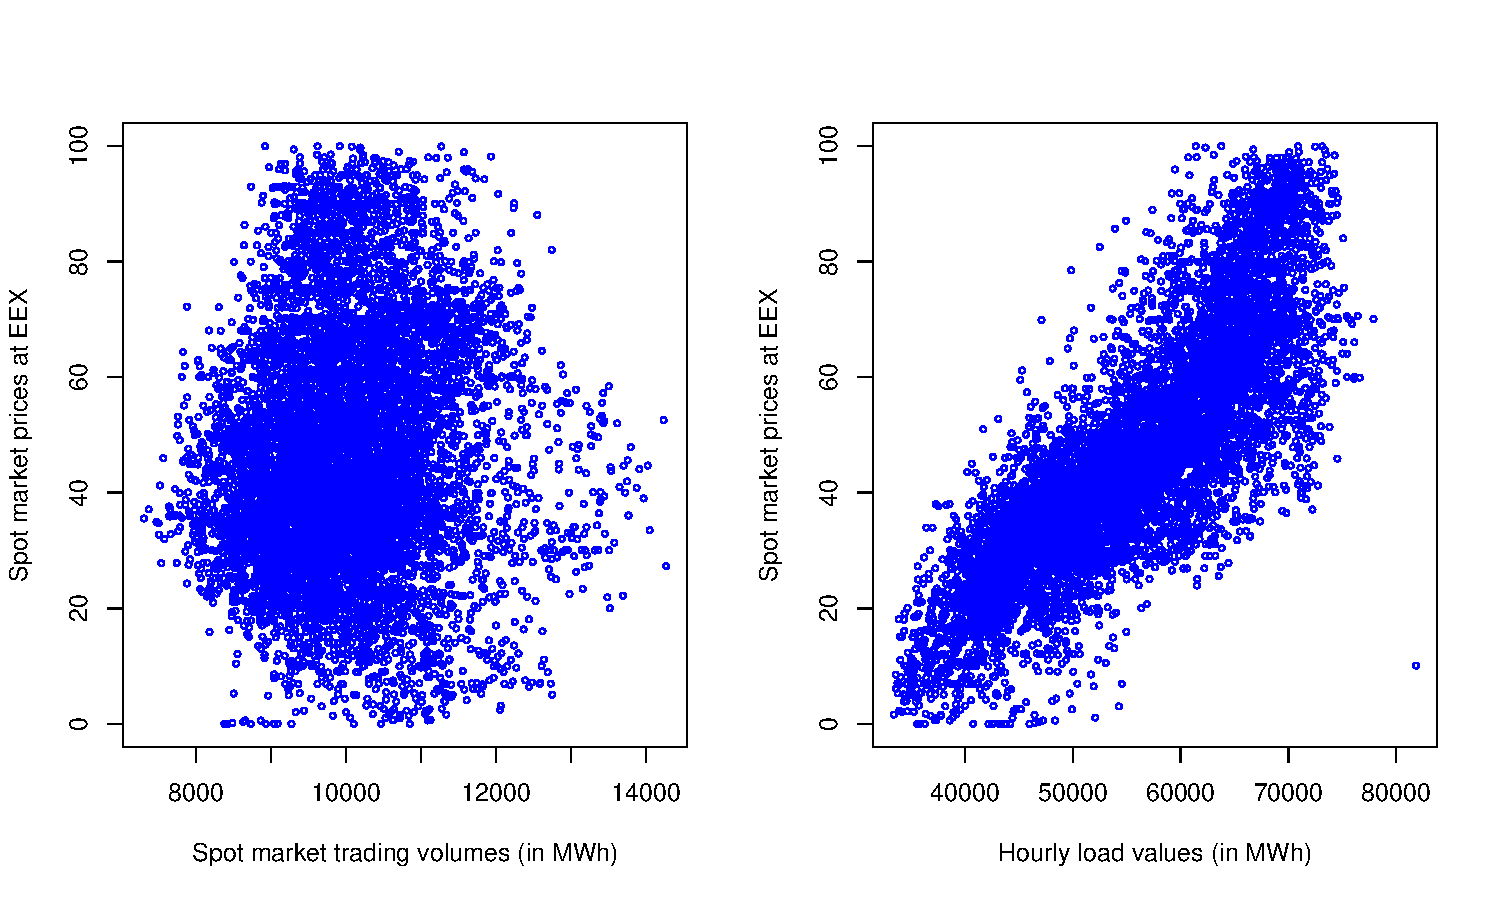
\includegraphics[width=3.5in]{germandata/pricequant.pdf}
  \label{fig:pricequant}
\\
 \scriptsize Source: EEX, UCTE
\end{figure}

To account for different states of the market we separated the price-quantity combinations which occurred within a year by prices. As can be seen in Table \ref{tab:demand}, markets with extremely high prices occur only seldomly and prices between 20 and 40 are most common. For each of the six states in which the market might be we created linear demand functions based on average prices and quantities in these states. Note, that we also model the high-price market segment, to include price spikes which are a stylized fact of electricity prices.  To construct demand curves, \cite{Neuhoff2005} use a demand elasticity of 0.1, whereby \cite{Genc2007} argue that 0.2 is more commonly used to simulate the electricity market. As we have a more long run focus, we decided to use the latter value. It might be argued, that electricity demand is completely inelastic, as maybe only a very few industrial clients reduce their demand when prices rise. In response to that, \cite{Bushnell2003} notes that imports and exports provide some elasticity.

\begin{table}[htb]
\centering
\caption{Market segments}
\vspace{0.3cm}
\begin{tabular}{lrrrr}
\hline
 & \multicolumn{1}{c}{Occupancy} & \multicolumn{1}{c}{Average price} & \multicolumn{1}{c}{Average quantity} &  \\ 
 & \multicolumn{1}{c}{per year} & \multicolumn{1}{c}{(EUR)} & \multicolumn{1}{c}{(MWh)} &  \\ 
 \hline
$>$ 100 & \multicolumn{1}{c}{46} & \multicolumn{1}{c}{128} & \multicolumn{1}{c}{83,558} &  \\ 
between 80 and 100 & \multicolumn{1}{c}{134} & \multicolumn{1}{c}{86} & \multicolumn{1}{c}{81,493} &  \\ 
between 60 and 80 & \multicolumn{1}{c}{788} & \multicolumn{1}{c}{68} & \multicolumn{1}{c}{78,256} &  \\ 
between 40 and 60 & \multicolumn{1}{c}{2,174} & \multicolumn{1}{c}{49} & \multicolumn{1}{c}{71,956} &  \\ 
between 20 and 40 & \multicolumn{1}{c}{4,201} & \multicolumn{1}{c}{30} & \multicolumn{1}{c}{58,578} &  \\ 
below 20 & \multicolumn{1}{c}{1,417} & \multicolumn{1}{c}{14} & \multicolumn{1}{c}{42,627} &  \\
\hline
 & \multicolumn{1}{c}{8760} &  &  &  \\ 
 \hline
\end{tabular}
\label{tab:demand}
\\
\vspace{0.3cm}
\scriptsize Source: UCTE and EEX 
\end{table}

%\subsection{Supply}

Data concerning the short run marginal costs and investment costs per MWh were obtained from \cite{Auer2006} and are shown in Table \ref{tab:costs}. For pump storage plants we used the real option value of peak load electricity, which we approximated by the average option price for peak load electricity at the EEX in the year 2006. We do not provide fixed costs for pump hydropower and oil plants. In the case of hydropower plants construction costs depend heavily on the respective sites and therefore such costs are hard to estimate. Furthermore, all available sites for significant hydropower capacities in Central Europe seem to be occupied already. Oil fired plants are not considered a relevant investment option, because oil prices are just too high. The fixed investment costs can also be interpreted as present value of future yearly costs of capital.

\begin{table}[htb]
\centering
\caption{Variable and fixed costs}
\vspace{0.3cm}
\begin{tabular}{rrr}
\hline
           & Variable Costs & Investment Costs \\

           & (EURO/MWh) & EUROs per MWh \\
\hline
     Hydro &        7.6 &    3,500,000 \\

   Nuclear &        9.5 &    1,841,000 \\

   Lignite &       10.6 &    1,074,000 \\

 Hard Coal &       16.1 &     971,000 \\

CCGT &       33.5 &     460,000 \\

Oil & 44            &   n.a.\\
%Gas Turbines &       53.8 &     332000 \\

Pump Hydro &         80 &       n.a.\\
\hline
\end{tabular}
\label{tab:costs}
\\
\vspace{0.3cm}
\scriptsize Source: \cite{Auer2006}
\end{table}



%%% Local Variables: 
%%% mode: latex
%%% TeX-master: "../eem08"
%%% End: 

\section{Optimal Capacity Expansion - Whats the Problem?}

\subsection{Peak load Pricing}

					\begin{frame}
					
\frametitle{Optimal Peak Load Pricing and perfect Competition}
\begin{columns}
\begin{column} {0.4\textwidth}

\begin{figure}[h]
\centering
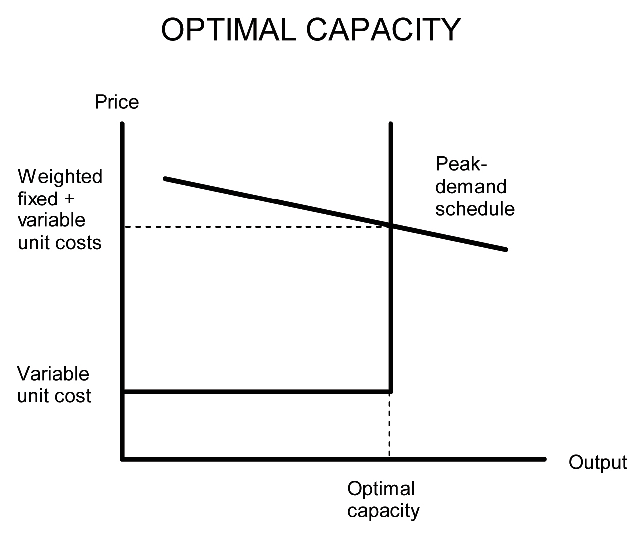
\includegraphics[width=1.\textwidth]{capacity/peak_load_opt}
    \caption{von der Fehr and Harbord (1994)}
    \label{fig:Daten 2004}            
\end{figure}
\end{column}

\begin{column} {0.6\textwidth}
\begin{itemize}
\item Optimal Capacity should be set such as to equate marginal benefits and costs from one unit of capacity
\end{itemize}

\begin{equation}
	c=(p^p-v)*\pi
\end{equation}

{\small
\begin{tabbing}
whereby: \= $c$ \  \= per unit cost of capacity \\
\> $p^p$   \    \> peak period price  \\
\> $v$    \   \> variable costs \\
\> $\pi$    \    \> chance to pave a peak period
\end{tabbing}}

\begin{itemize}
\item Which is exactly what a perfectly competitive firm would do
\end {itemize}

\begin{itemize}
\item Note that we assume price rationing and no rationing costs
\end {itemize}

\end{column}
\end{columns}

							\end{frame}
							\begin{frame}

\frametitle{Distorted Incentives under imperfect Competition I}
\begin{columns}
\begin{column} {0.4\textwidth}

\begin{figure}[h]
\centering
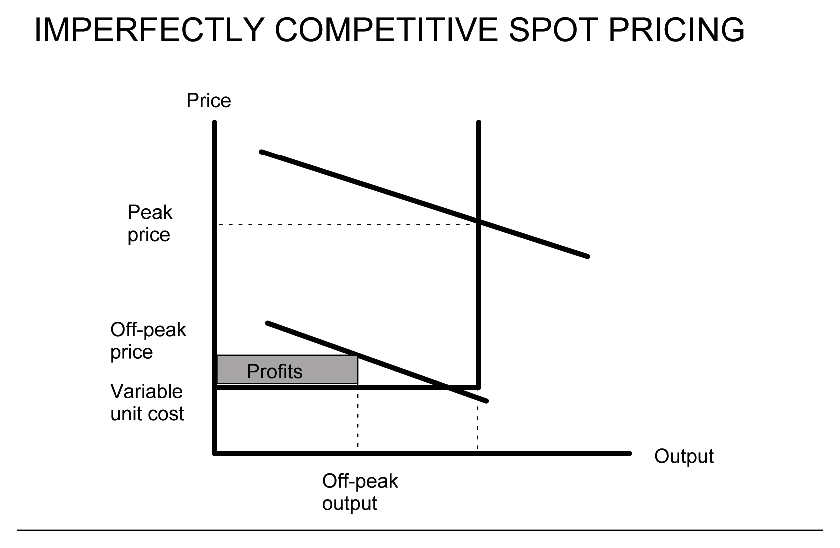
\includegraphics[width=1.\textwidth]{capacity/peak_load_toohigh}
    \caption{von der Fehr and Harbord (1994)}
    \label{fig:Daten 2004}            
\end{figure}
\end{column}

\begin{column} {0.6\textwidth}
\begin{itemize}
\item prices $>$ marginal costs in off peak periods 
\item additional incentive to invest by a possible gain during off peak periods if capacity allows to steal business
\end {itemize}
  
\begin{equation}
	1/2 (1-\pi) (p^{op}-v)
\end{equation} 
{\small
\begin{tabbing}
whereby: \= $p^{op}$ \  \= off peak price
\end{tabbing}}

\begin{itemize}
\item the social optimality condition is the same as before
\item distortion toward too much investment
\end {itemize}

\end{column}
\end{columns}
	

							\end{frame}
							\begin{frame}

\frametitle{Distorted Incentives under imperfect Competition II}
\begin{columns}
\begin{column} {0.4\textwidth}

\begin{figure}[h]
\centering
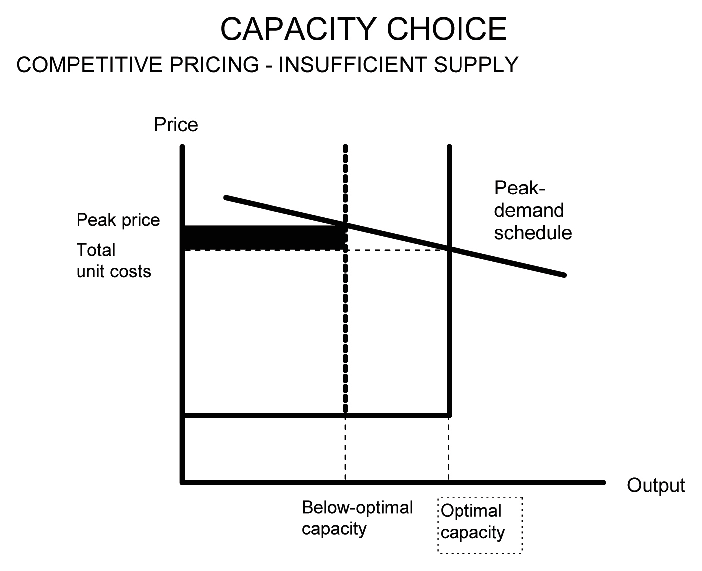
\includegraphics[width=1.\textwidth]{capacity/peak_load_insufficient}
    \caption{von der Fehr and Harbord (1994)}
    \label{fig:Daten 2004}            
\end{figure}
\end{column}

\begin{column} {0.6\textwidth}
\begin{itemize}
\item there might be an incentive to cut investments to drive up the price in peak periods
\end {itemize}

\begin{equation}
\pi (w^p(K)+\frac{\partial w^p(K)}{\partial q}-v)
\end{equation}

{\small
\begin{tabbing}
\= $w^p$ \  \= peak period demand function \\
\> $K$   \    \> capacity
\end{tabbing}}

\begin{itemize}
\item as we switched to imperfect competition, the change in price induced by more capacity has to be accounted for
\item as this effect is negative, incentives to invest are distorted downwards
\end {itemize}

\end{column}
\end{columns}
	

			\end{frame}

\subsection{Optimal Technology Mix}

			\begin{frame}

\frametitle{The optimal Technology Mix I}
\begin{columns}
\begin{column} {0.4\textwidth}

\begin{figure}[h]
\centering
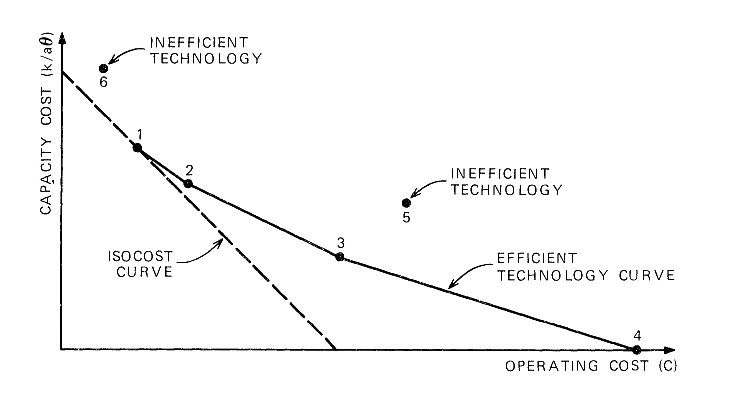
\includegraphics[width=1.\textwidth]{capacity/technology_choice_chow}
    \caption{Chau (1983)}
    \label{fig:Daten 2004}            
\end{figure}
\end{column}

\begin{column} {0.6\textwidth}
\begin{itemize}
\item how to choose the optimal technology?
\item different possible combinations of capacity and operating costs
\item by using a standard isocost line one could get the cheapest technology
\item does not work if demand is uncertain or variable
\item some idle capacity inevitable
\item less capital intensive technologies become attractive
\end {itemize}

\end{column}
\end{columns}


			\end{frame}			
			\begin{frame}

\frametitle{The optimal Technology Mix II}
\begin{columns}
\begin{column} {0.4\textwidth}

\begin{figure}[h]
\centering
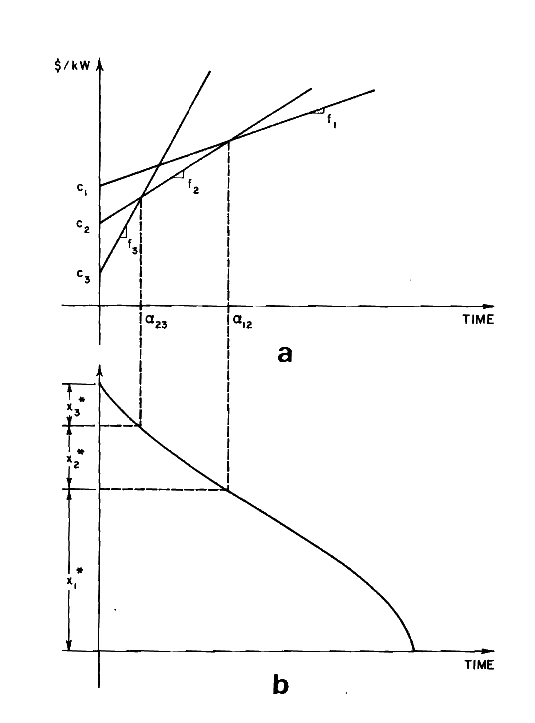
\includegraphics[width=1.\textwidth]{capacity/technology_choice_sherali}
    \caption{Chau (1983)}
    \label{fig:Daten 2004}            
\end{figure}
\end{column}

\begin{column} {0.6\textwidth}
\begin{itemize}
\item the load duration curve (\textbf{b}) plots the hours of the year ordered according to their energy demand
\item \textbf{(a)} shows three different cost curves each is cheaper for a certain yearly running time
\item technology 3 covers peak demand most efficiently 
\item but if it would run more than $\alpha_{23}$ hours of the year, technology two would be cheaper already
\item analogously, technology one is best used for base load
\end {itemize}

\end{column}
\end{columns}


			\end{frame}	
%\newpage
\section{The model}

\subsection{Static model - peak load pricing}

We begin with a static version of our model to establish the link to the economic intuition outlined in the previous section. There are four players, indexed by $i\in N$ (RWE, EON, Vattenfall and EnBW), seven technologies $k\in K$  and six different market states $m\in M$. Each of the players maximizes the following profit function:

\begin{gather}
	\max \pi_i(q_{i,k}^m,K_{i,k},)= \sum_{m\in M} v_m\times\\ \nonumber  \left[(\alpha_m-\beta_m\sum_{i\in N} \sum_{k\in K} q_{i,k}^m ) \sum_{k\in K} q_{i,k}^m - \sum_{k\in K} c^k q_{i,k}^m \right] \\ \nonumber
			\text{s.t.:} \  q_{i,k}^m-K_{i,k} \leq 0;\  \forall i,k,m \\
 										  q_{i,k}^m	\geq 0; \ \forall i,k,m   \nonumber
\end{gather}

\begin{tabular}[c]{l l}
$i\in N$        & players, firms\\
$s\in S$       	& scenarios\\
$m\in M$	& states of the market \\
$k\in K$	& technologies \\
$t\in T$	& time \\
$K_{i,k}^t$      & available capacity at time $t$ from technology $k$ \\
                & for firm $i$ \\
$q_{i,k}^{s,m,t}$ & quantity produced at time $t$ with technology $k$\\
                 &by firm $i$ in market state $m$ and scenario $s$ \\			
$I_{i,k}^t$   & investment in technology $k$ at time $t$  \\
              & by firm $i$\\
$p_s$        & probability of scenario $s$\\
$\nu_m$      & says how often (how many hours) market \\
             & state $m$ occurs \\
$\delta$   & discount factor \\
$\rho$   & depreciation factor \\
$\alpha_m$  & demand function intercept in market state $m$ \\
$\beta_m$   & demand function slope in market state $m$ \\
$c_k$	     & variable costs of technology $k$	\\
$\Gamma_k$   & investment costs in technology $k$  \\
$F_k$        & scrap values  \\
\\
\end{tabular}

$\alpha_m$ and $\beta_m$ are the intercept and the slope of the inverse demand function in the different market states derived from Table \ref{tab:demand}. $q_{i,k}^m$ is the quantity produced with each technology by each player in each market state and $K_{i,k}$ is the corresponding capacity which is now given for each player as we are solving for the short run equilibrium. $c_k$ are the short run variable costs which are the same for each producer. The parameter $\nu_m $ says how often a certain demand state occurs. This parameter is used as a weight for the shadow price of capacity. We derived the Karush Kuhn Tucker (KKT) conditions to obtain a mixed complementarity problem (MCP) and solved it by using the PATH Solver in GAMS.

Table \ref{tab:statquant} in the appendix shows the quantities predicted by our oligopoly model. While during a high demand state almost all capacities are used, during low demand states hard coal plants are the most expensive technology in the merit order curve. Prices differ significantly but are above marginal costs even if demand is very low. Please note, that there is strategic capacity withholding as not all capacities are brought to the market even if more than the variable costs were covered.

As we used a Lagrangian method to calculate this short run equilibrium, we can have a look at the shadow prices of capacity to see how much an additional unit of capacity would be worth for each player. Please note that this values cannot be smaller than zero as, in our setup, there always exists the option of not using existing capacities. There are only positive scarcity rents if the capacity of the technology is binding. Table \ref{tab:statlambda} shows the shadow prices of capacity. The values can be read in such a way that an additional MW of hydro power capacity would increase profits RWE makes in all the extremely high market states by 831 Euros and the overall yearly profit of RWE by 44,832 EUROS. On the contrary, the same capacity is worth 269,972 Euros for EnBW. How can such different results be explained? One the one hand, it seems that firms gain less from investing during high demand states which is straightforward as demand is more inelastic during high demand states and so one looses more by adding more capacity which depresses the gain from capacity. On the other hand, there are positive values for almost all technologies during extremely high demand states as most of the capacities become binding then. \\
Most importantly, for smaller players like Vattenfall and EnBW shadow prices are far higher as the effect of less scarcity, and thereby lower prices is less important if firms sell less. This means that it is impossible to assess the investment incentives for firm on a market like the electricity market (oligopoly with $L$-shaped cost functions) without considering the strategic implications such investments have.

\subsection{Dynamic model}

In this part, we introduce two deciding factors. First, dynamics and thereby investments which link the different time periods. Second, uncertainty which is accounted for by a binomial scenario tree and leads to a recourse problem. The uncertainty about future demand is accounted for by different demand scenarios. Our approach follows the game with probabilistic scenarios (GPS) method by \cite{Genc2007}. Our two stage Model looks as follows.

\begin{gather}
	\max \pi_i(q_{i,k}^{s,m,t},K^t_{i,k},I_{i,k})=	\\ \nonumber 
	\sum_{m\in M} v_m \left[ (\alpha_m^l-\beta_m^l \sum_{i\in N}\sum_{k\in K} q_{i,k}^{l,m,1}) \sum_{k\in K} q_{i,k}^{l,m,1} - \sum_{k\in K} c_k q_{i,k}^{l,m,1} \right]  \\  \nonumber 
	+ \delta \sum_{s\in S} p_s \sum_{m\in M} v_m \times \\ \nonumber \left[ (\alpha_m^s-\beta_m^s \sum_{i\in N}\sum_{k\in K} q_{i,k}^{s,m,2}) \sum_{k\in K} q_{i,k}^{s,m,2} - \sum_{k\in K} c_k q_{i,k}^{s,m,2}  \right]   \\  \nonumber 
									- \sum_{k\in K} \Gamma_{k\in K} I_{i,k} + \delta \sum_{k\in K} F_k I_{i,k}  \\       
			\text{s.t.:} \  q_{i,k}^{l,m,1} - K^{1}_{i,k} \leq 0; \ \forall i,k,m    \label{eq:oligopmax2}\\ 
											q_{i,k}^{s,m,2} - K^{2}_{i,k} \leq 0; \ \forall i,k,m,s  \label{eq:oligopmax3}\\
										  K^{2}_{i,k}  - \rho K^{1}_{i,k}  - I_{i,k} = 0 ; \ \forall i,k  \label{eq:ologopmax5} \\  
 										  q_{i,k}^{s,m,t};K^t_{i,k};I_{i,k}	\geq 0; \ \forall i,k,s   \nonumber
\end{gather}

Each player maximizes its profit by setting $q_{i,k}^{s,m,t}$ and $I_{i,k}^t$. By considering different demand scenarios ($s\in S$) and the associated probabilities ($p_s$), the players take into account how demand might evolve in the future. Capacities now evolve over time $t\in T$ according to the state equation \eqref{eq:ologopmax5}. The capacity constraints are given in \eqref{eq:oligopmax2} and \eqref{eq:oligopmax3}. Quantities are allowed to adapt to the scenarios, thereby accounting for the fact that firms can always react to demand by adjusting their short run production. On the contrary, investments are not allowed to differ in such a way as they have to be set in advance when it is not clear yet how high demand might be. Please note, that quantities do not depend on what other players might invest. They do depend however, on how high own investments are. 
% as the cost function can be changed between period one and two($C^1_i vs. C^2_i$). (Idee - Wenn man das weggibt, m�sste man den Effekt den eigene Investments auf den Marktpreis haben sehen). 
If quantities would depend on investments of other players as well, we would enter the realm of feedback or closed loop games (which are the same in the case of a two-stage game). It has to be noted here that the solution of a closed loop game can, and will, in general, be different from the solution of an open loop game.

To solve the model, we derive the KKT conditions to obtain an MCP problem which we solve by using GAMS and the PATH solver. For the model above, we used the Cournot approach to derive the first order conditions. For the competitive benchmark we solved the problem under the assumption that just one welfare maximizing player disposes of all the initial capacities of the four players. When deriving the KKT conditions, for the optimal results this player is assumed to set prices equal to marginal costs.
%\clearpage




%%% Local Variables: 
%%% mode: latex
%%% TeX-master: "../eem08"
%%% End: 

%\section{Data}

Austrian and German electricity market are integrated. Therefore, we need data for the major players in both countries. There are no serious network congestions on the border between Austria and Germany. (for reference see Todem)

For the supply we need for every player

\begin{itemize}
\item variable and fixed costs,
\item structure of the plant park.
\end{itemize}

Parameters for the demand curve are obtained from

\begin{itemize}
\item load duration curve
\item how parameters for demand functions from load duration curve
\end{itemize}

Show that Austrian players are fringe? 

Long term structure of plant parks.

How does the resulting plant park structure look like, if firms actually play two-stage open or closed-looped games and other possible market structures (perfect competition, Betrand). 

How could the current market structures look like one long term step ahead (in ten years from now, one investment cycle).

Welfare implications from different market structures.

Implications of capacity markets.


%\section{Ideas}

\begin{itemize}
	\item \cite{Pineau2003} study how electricity prices, production levels and production capacities unfold in \emph{absence of regulation}. Why test different regulatory measures in this game theoretic setting?
	\item Can transmission pricing and constraints also be ignored in Austria?
	\item Parameters to check in sensitivity analysis: depreciation rate of generating capacity
\end{itemize}



%------------------------------------------------------

\markboth{References}{References} %\frenchspacing
\bibliographystyle{chicago}
%\nocite{*}
\bibliography{microsim}

%\appendix
%\newpage
%\section*{Appendix}
%\begin{landscape}

\begin{table}
\scriptsize
\begin{tabular}[h]{ccccc}
\hline
\textbf{Investment problem}\\
\hline
  Authors & Information structure & Solution method & Transmission network & Numerical application \\
\hline
\cite{Genc2007} & $S$-adapted open-loop & MCP & No & electricity market, Ontario, Canada\\
1 & 2 & 3 & 4 & 5 \\
\hline
\textbf{Stochastic oligopoly models}\\
\hline
\cite{Salant1982}\\
\cite{Wolf1997}\\
\cite{Haurie2001}\\
\cite{Haurie2002}\\
\cite{Murto2004}
\end{tabular}
\end{table}
bla ble blu


\textbf{References:} \cite{Salant1982, Wolf1997, Haurie2001, Haurie2002, Pineau2003, Murto2004}\\


The $S$-adapted information structure was introduced by \cite{Haurie1990}.
$S$-adapted structure is similar to the open-loop case, except that the strategies of the players adapt to the sample path of the stochastic variable \citep[see][pg. 128]{Pineau2003}.

\cite{Haurie2002} developed an approximation method with variational inequalities for $S$-adapted oligopoly equilibria. It can be used with any discrete state process that can be represented as an event tree can be used as description of the random disturbances.

\cite{Murto2004} solves the game with feedback information structure.

\cite{Haurie2001}, \cite{Genc2007}

developed an approximation method with variational inequalities for $S$-adapted oligopoly equilibria. It can be used with any discrete state process that can be represented as an event tree can be used as description of the random disturbances.


Market simulation: \cite{Torre2003}, \cite{Valenzuela2007}, \cite{Hobbs2001},\cite{Otero-Novas2000}

General review paper: \cite{Neuhoff2005}, \cite{Ventosa2005}, \cite{Kahn1998}

\end{landscape}



%%% Local Variables: 
%%% mode: latex
%%% TeX-master: "../emarket_simulation"
%%% End: 

%
\begin{table}[htb]
\centering
\caption{quantities offered and market prices by different firms in different market states}
% Table generated by Excel2LaTeX from sheet 'Tabelle1'
\begin{tabular}{llrrrrrr}
\hline
\hline
           &            & extr. high &    v. high &       high &    interm. &        low &     v. low \\
\hline
       RWE & Hydro Power &        741 &        741 &        741 &        741 &        741 &        741 \\

           &    Nuclear &       5,499 &       5,499 &       5,499 &       5,499 &       5,499 &       5,499 \\

           &    Lignite &      10,554 &      10,554 &      10,554 &      10,554 &      10,285 &       3,684 \\

           &  Hard Coal &       7,249 &       7,249 &       6,675 &       3,124 &            &            \\

           &  {\bf Sum} & {\bf 24,043} & {\bf 24,043} & {\bf 23,469} & {\bf 19,918} & {\bf 16,525} & {\bf 9,924} \\
\hline
       EON & Hydro Power &       1,320 &       1,320 &       1,320 &       1,320 &       1,320 &       1,320 \\

           &    Nuclear &       8,473 &       8,473 &       8,473 &       8,473 &       8,473 &       8,473 \\

           &    Lignite &       1,425 &       1,425 &       1,425 &       1,425 &       1,425 &        131 \\

           &  Hard Coal &       9,461 &       9,461 &       9,461 &       8,700 &       3,133 &            \\

           &        Gas &       2,340 &       1,238 &            &            &            &            \\

           &  {\bf Sum} & {\bf 23,019} & {\bf 21,917} & {\bf 20,679} & {\bf 19,918} & {\bf 14,351} & {\bf 9,924} \\
\hline
Vattenfall & Hydro Power &          9 &          9 &          9 &          9 &          9 &          9 \\

           &    Nuclear &       1,421 &       1,421 &       1,421 &       1,421 &       1,421 &       1,421 \\

           &    Lignite &       6,932 &       6,932 &       6,932 &       6,932 &       6,932 &       6,932 \\

           &  Hard Coal &       1,729 &       1,729 &       1,729 &       1,729 &       1,729 &            \\

           &        Gas &        870 &        870 &        870 &        870 &            &            \\

           &        Oil &       1,429 &       1,429 &       1,429 &        702 &            &            \\

           &   Pump St. &       2,883 &        702 &            &            &            &            \\

           &  {\bf Sum} & {\bf 15,273} & {\bf 13,092} & {\bf 12,390} & {\bf 11,663} & {\bf 10,091} & {\bf 8,362} \\
\hline
      EnBW & Hydro Power &        447 &        447 &        447 &        447 &        447 &        447 \\

           &    Nuclear &       4,272 &       4,272 &       4,272 &       4,272 &       4,272 &       4,272 \\

           &    Lignite &        453 &        453 &        453 &        453 &        453 &        453 \\

           &  Hard Coal &       3,288 &       3,288 &       3,288 &       3,288 &       3,288 &       1,465 \\

           &        Gas &       1,083 &       1,083 &       1,083 &       1,083 &            &            \\

           &        Oil &        617 &        617 &        617 &        617 &            &            \\

           &   Pump St. &        368 &        368 &            &            &            &            \\

           &  {\bf Sum} & {\bf 10,528} & {\bf 10,528} & {\bf 10,160} & {\bf 10,160} & {\bf 8,460} & {\bf 6,637} \\
\hline
           &    ov. Sum & {\bf 72,863} & {\bf 69,580} & {\bf 66,698} & {\bf 61,660} & {\bf 49,427} & {\bf 34,847} \\
\hline
           &      Price &  {\bf 210} &  {\bf 149} &  {\bf 118} &   {\bf 83} &   {\bf 52} &   {\bf 27} \\
\hline
\hline
\end{tabular}
\label{tab:statquant}
\begin{center}
Source: own calculations
\end{center}
\end{table}

\clearpage
\newpage
%\vspace{3cm}
\begin{table}[htb]
\centering
\caption{shadow prices of capacity, separated by technologies and market states}
% Table generated by Excel2LaTeX from sheet 'Tabelle1'
\begin{tabular}{llrrrrrrr}
\hline
           &            & extr. high &    v. high &       high &    interm. &        low &     v. low &  {\bf Sum} \\
\hline
       RWE & Hydro Power &        831 &       1970 &       6698 &      18479 &      12603 &       4251 & {\bf 44832} \\

           &    Nuclear &        743 &       1715 &       5201 &      14348 &       4621 &       1559 & {\bf 28188} \\

           &    Lignite &        693 &       1568 &       4334 &      11957 &            &            & {\bf 18552} \\

           &  Hard Coal &        440 &        831 &            &            &            &            & {\bf 1271} \\
\hline
       EON & Hydro Power &       1191 &       3471 &      16261 &      18479 &      35709 &       4251 & {\bf 79362} \\

           &    Nuclear &       1104 &       3216 &      14764 &      14348 &      27727 &       1559 & {\bf 62718} \\

           &    Lignite &       1053 &       3069 &      13897 &      11957 &      23106 &            & {\bf 53082} \\

           &  Hard Coal &        800 &       2332 &       9563 &            &            &            & {\bf 12695} \\
\hline
Vattenfall & Hydro Power &       3917 &       9702 &      44668 &      79134 &      81002 &       7954 & {\bf 226377} \\

           &    Nuclear &       3830 &       9447 &      43171 &      75003 &      73020 &       5262 & {\bf 209733} \\

           &    Lignite &       3779 &       9300 &      42304 &      72612 &      68399 &       3703 & {\bf 200097} \\

           &  Hard Coal &       3526 &       8563 &      37970 &      60655 &      45293 &            & {\bf 156007} \\

           &        Gas &       2726 &       6231 &      24259 &      22827 &            &            & {\bf 56043} \\

           &        Oil &       2243 &       4824 &      15985 &            &            &            & {\bf 23052} \\

           &   Pump St. &        587 &            &            &            &            &            &  {\bf 587} \\
\hline
      EnBW & Hydro Power &       5587 &      11512 &      52311 &      90176 &      98341 &      12045 & {\bf 269972} \\

           &    Nuclear &       5500 &      11257 &      50814 &      86045 &      90359 &       9352 & {\bf 253328} \\

           &    Lignite &       5449 &      11110 &      49947 &      83654 &      85738 &       7794 & {\bf 243692} \\

           &  Hard Coal &       5196 &      10373 &      45613 &      71697 &      62633 &            & {\bf 195512} \\

           &        Gas &       4396 &       8041 &      31902 &      33869 &            &            & {\bf 78208} \\

           &        Oil &       3913 &       6634 &      23628 &      11042 &            &            & {\bf 45217} \\

           &   Pump St. &       2257 &       1810 &            &            &            &            & {\bf 4067} \\
\hline
\hline
\end{tabular}  
\label{tab:statlambda}
\begin{center}
Source: own calculations
\end{center}
\end{table}
\end{document}

%%% Local Variables: 
%%% mode: latex
%%% TeX-master: t
%%% End: 
